\documentclass[11pt]{article}
\usepackage{xspace}
\usepackage[ngerman,english]{babel}
\usepackage{graphicx,lipsum}
\usepackage[europeanvoltages,
europeancurrents,
europeanresistors,
americaninductors,
smartlabels,siunitx,straightvoltages]{circuitikz}
\usepackage{float}
%Here we define a marco: The \xspace ensures correct spacing, i.e. insert space before next word, but not before period or comma.
\newcommand{\paxos}{\textsc{Paxos}\xspace}

%These packages are needed for the plot in Figure 1. 
\usepackage{tikz}
\usepackage{pgfplots}
\pgfplotsset{compat=newest}



% Use option lineno for line numbers 
\allowdisplaybreaks

\begin{document}
\selectlanguage{ngerman} 
%\flushbottom
%\maketitle
%\thispagestyle{empty}

\section{Introduction}

\subsection{Widerstandsmessung}
Bei dieser Aufgabe, wurden die Widerstandswerte der Primär- und Sekundärseite aus den bemessenen Strom und Spannung der Wicklungen bestimmt. \par

Die Widerstände jedes Strangs wurde berechnet und daraus wurde der Mittelwert gebildet. 
Die folgenden Werte für $R_1$ und $R_2$ wurden erhalten:
\begin{table}[H]
\centering
\begin{tabular}{@{}llll@{}}
\toprule
\multicolumn{1}{c}{Wicklung} & \multicolumn{1}{c}{U} & \multicolumn{1}{c}{I} & \multicolumn{1}{c}{R} \\ \midrule
Up                           & 0.29                  & 0.48                  & 0.60                  \\
Vp                           & 0.30                  & 0.49                  & 0.62                  \\
Wp                           & 0.30                  & 0.50                  & 0.62                  \\
Us                           & 0.29                  & 0.83                  & 0.35                  \\
Vs                           & 0.20                  & 0.83                  & 0.24                  \\
Ws                           & 0.20                  & 0.83                  & 0.24                  \\ \bottomrule
\end{tabular}%
\caption{SOME CATOPN}
\label{tab:my-table}
\end{table}
\begin{align*}
    R_1 &= \SI{0.61}{\ohm} \\ R_2 &= \SI{0.28}{\ohm}
\end{align*}




%TODO LEERLAUF VEERSUCH 
\subsection{Leerlaufversuch}
In dieser Messaufgabe, wurde die primärseitige Spannung mittels eines Stelltransformators variiert. Durch erhöhung dieser Spannung mit Schritten von 40 V, wurde die sekundärseitige Spannung bis der Bemessungswert von $U_{1L} = 400 \text{V}$ erreicht wurde bemessen. Der Strom der bei der Bemessungsspannug auftaucht (auch Leerlaufstrom genannt) einschließlich der Wirkleistung wurden auch bemessen und dokumentiert. \par  
Die Messschaltung für diese Schaltung is in der unteren Abbildung dargestellt. \par 
\begin{figure}[H]
    \centering
    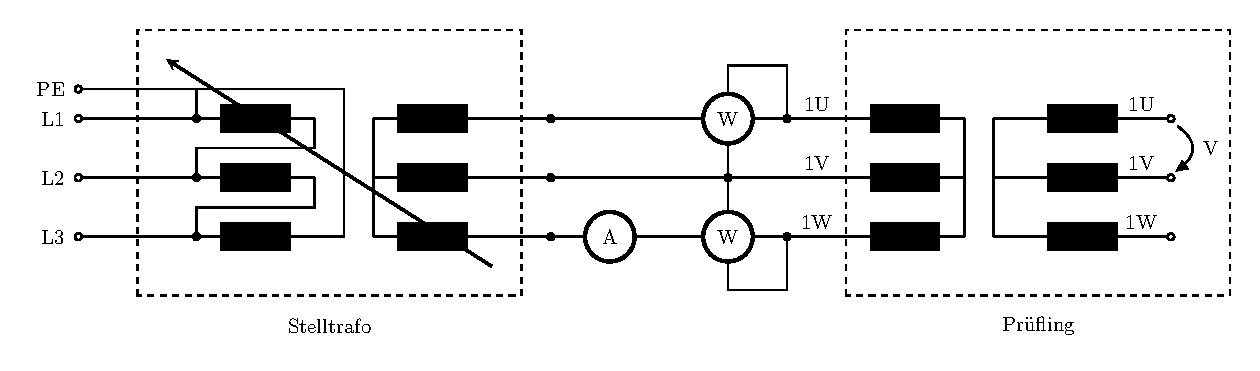
\includegraphics[width=0.95\textwidth]{fig/ll_mess.pdf}
    \caption{Messschaltung Leerlaufversuch }
\end{figure}
 Die Abhängigkeiten $U_{2L} = f(U_{1L}) $ und $ \text{ü} = f(U_{1L})$ sind in den unten stehenden Diagrammen dargestellt.  \par 
% LEERLAUF U_1L vs U_2L
  \begin{figure}[H]
	\begin{subfigure}{0.48\textwidth}
	  \centering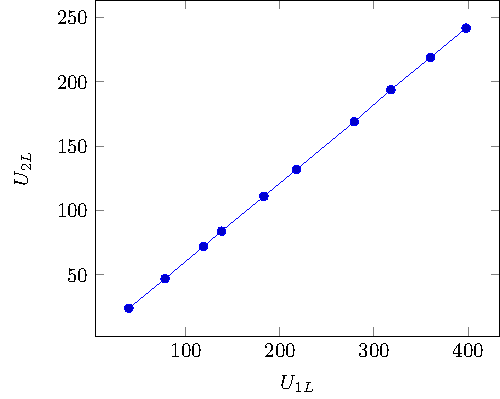
\includegraphics[width=0.95\textwidth]{fig/ll_u1ue.pdf}
	\end{subfigure}
	\begin{subfigure}{0.48\textwidth}
	  \centering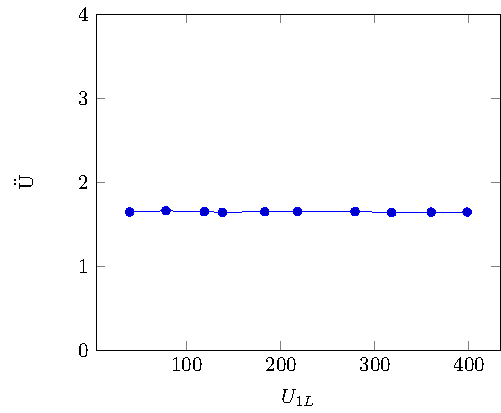
\includegraphics[width=0.95\textwidth]{fig/ll_ue.pdf}
	\end{subfigure}
	\caption{$U_{2L}$ (\si{\volt})  und Übersetzungsverhältnis ü in Abhängigkeit von $U_{1L}$ (\si{\volt})  }
  \end{figure}
  
Zusätzlich wurden die folgenden Werte bei  $U_{1L} = 400 \text{V}$ erhalten: \\
\begin{align*}
  \intertext{Leerlaufstrom: } I_{l} &=  \SI{472.1}{\milli\ampere}  \\  
  \intertext{Wirkleistung: }
 P_l &= P_{UV} + P_{VW}  \\
&=  \SI{-98}{\watt} + \SI{160}{\watt}\\
&=  \SI{62}{\watt}    \\
\intertext{Übersetzungsverhältnis:} \text{ü} &= \frac{U_{1L}}{U_{2L}} \\&= \frac{ \SI{398}{\volt}}{ \SI{241.9}{\volt} } \\
&= 1.65 \\
\intertext{Eisenstrom: } I_{Fe} &=
\frac{P_l}{U_{1L}} \\
&=  \SI{90}{\milli \ampere}  \\
\intertext{Hauptflussstrom: } I_{H} &=
\sqrt{I_{1L}^2-I_{Fe}^2} \\
&=  \SI{463.45}{\milli \ampere}\\
\intertext{Eisenwiderstand: } R_{Fe} &= \frac{U_{1L}}{\sqrt{3}\cdot I_Fe} \\
&= \frac{ \SI{398}{\volt}}{ \SI{90}{\milli\ampere} } \\
&= \SI{2.55}{\kilo\Omega}\\
\intertext{Hauptinduktanz: } X_{h} &= \frac{U_{1L}}{\sqrt{3} \cdot I_{\mu} } \\
&= \frac{ \SI{398}{\volt}}{ \sqrt{3}\cdot \SI{463.45}{\milli\ampere} } \\
&= \SI{0.496}{\kilo \Omega}  \\
\intertext{Leistungsfaktor: } cos(\varphi) &= \frac{\sqrt{3}*P_l}{3*U_{1L}*I_{1L}} \\
&=  0.19
\end{align*}

\begin{figure}[H]
    \centering
    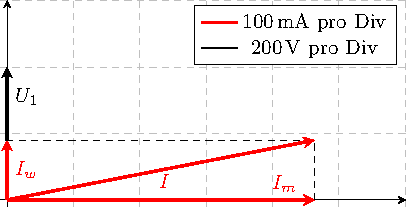
\includegraphics{fig/phasor_open.pdf}
    \caption{Caption}
    \label{fig:open}
\end{figure}

%TODO KS VEERSUCH 

\subsection{Kurzschlussversuch}

In dieser Versuchsaufgabe wird bei kurzgeschlossener Sekundärwicklung die Eingangsspannung mit Hilfe eines Stelltransformators
so weit erhöht, bis der Nennstrom fließt.
In diesem Versuch sind die Eisenverluste vernachlässigbar klein,
Mit dem Leistungsmesser werden bei Kurzschluss somit die Kupferverluste  gemessen.

\par 
Die verwendete Messschaltung ist unten Abbgebildet.  \par
\begin{figure}[h]
    \centering
    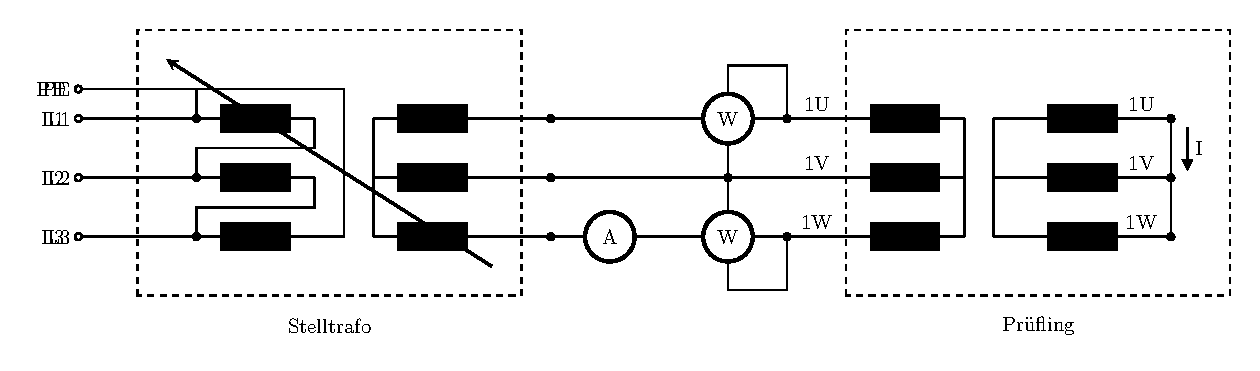
\includegraphics[width=0.95\textwidth]{fig/kz_mess.pdf}
    \caption{Messschaltung Kurzschluß}
    \label{fig:my_label}
 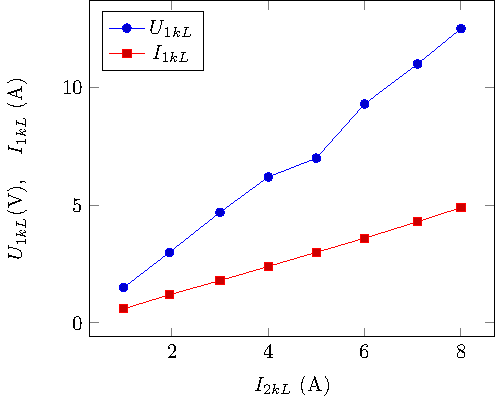
\includegraphics{fig/kz.pdf}
    \caption{Kurzschlussspannung und primärseitiger Kurzschlußstrom in Abhängigkeit von sekundärseitigem Kurzschlußstrom}
\end{figure}

\begin{align*}
\cos \phi_k &= \frac{P_k}{\sqrt{3}U_{1kL} \cdot I_{1k\varphi}}\\
&= \frac{75}{\sqrt{3}\cdot 4.9 \cdot 12.5} \\
&= 0.707\\
    Z_k &= \frac{V}{I}\\
    & = \SI{1.56}{\ohm}\\
    R_{k} &= \frac{P}{3 \cdot I_{\varphi}^2} = Z \cdot \cos \phi\\
    &=1.56 \cdot 0.707 \\
    &= \SI{1.04}{\ohm}\\
   X_k &= \SI{1.18}{\ohm}\\
    u_k &= \frac{U_{1k}}{U_{1B}}\cdot 100 \% \\
    &= \frac{12.5}{400}\cdot 100 \% \\
    & = \SI{3.125}{\percent}
\end{align*}
\begin{align*}
    R^\prime_2 &= \text{Ü}^2 \cdot R_1\\
    &= 1.73^2 \cdot 0.28 = \SI{0.83}{\ohm} \\ 
    X_k &= X_{\sigma 1} +   X_{\sigma 1} \cdot \frac{ R^\prime_2 }{R_1}\\
    X_{\sigma 1} &= \dfrac{X_k}{1+\dfrac{ R^\prime_2 }{R_1}}\\
     X_{\sigma 1} &= \dfrac{1.18}{1+\dfrac{0.83}{0.61}}\\
     &= \SI{0.5}{\ohm}\\
      X^\prime_{\sigma 2} &= \SI{0.68}{\ohm}
\end{align*}

\begin{figure}[H]
    \centering
    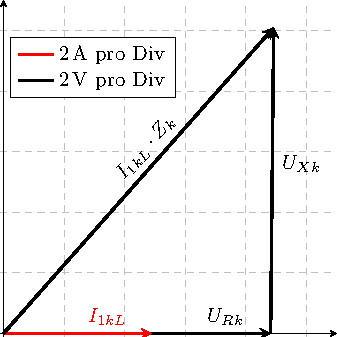
\includegraphics{fig/phasor_short.pdf}
    \caption{Caption}
    \label{fig:open}
\end{figure}

\subsection{Ohmische Belastung}
In dieser Versuchsaufgabe, wurde ein regelbarer Widerstand an jedem Strang der Sekundärwicklung angeschlossen. Beginnend mit einem Widerstandswert der einen Sekundärstrom von 1 A ergab, wurden die Widerstände   in Schritten von 1 A symmetrisch verändert bis 8 A erreicht wurde. \par
$I_{1L}$, $U_{2L}$, $\eta$ und cos($\varphi$) in Abhänigkeit von $I_{2L}$  sind unten dargestellt. 
\begin{figure}[H]
    \centering
    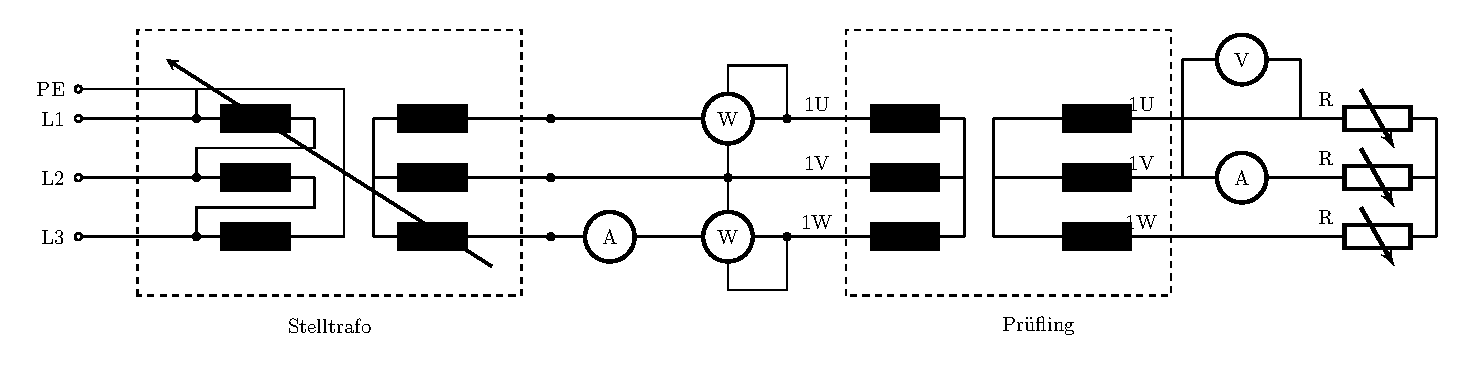
\includegraphics[width=0.95\textwidth]{fig/ohm_mess.pdf}
    \caption{Messschaltung Ohmische Belastung }
    \label{fig:my_label}
\end{figure}
\begin{figure}[H]
    \centering
	\begin{subfigure}{6cm}
	  \centering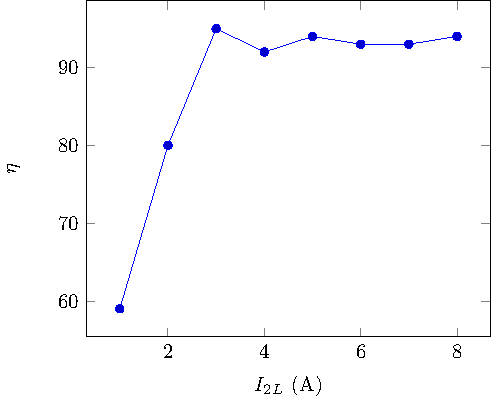
\includegraphics[width=6cm]{fig/r_eta.pdf}
	\end{subfigure}
	\begin{subfigure}{6cm}
	  \centering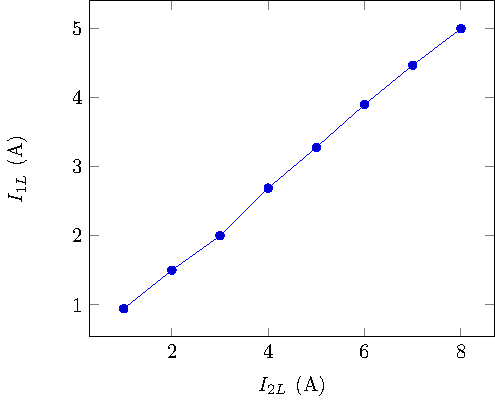
\includegraphics[width=6cm]{fig/r_i1i2.pdf}
	\end{subfigure}

	\begin{subfigure}{6cm}
	  \centering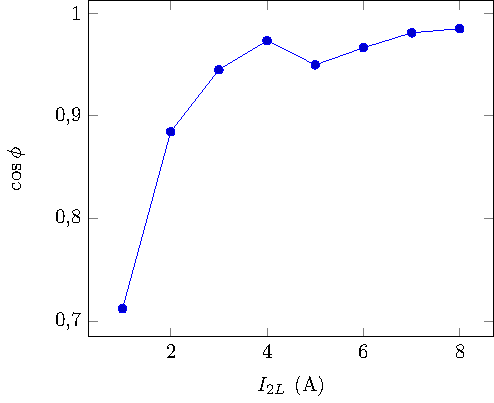
\includegraphics[width=6cm]{fig/r_pf.pdf}
	\end{subfigure}
	\begin{subfigure}{6cm}
	  \centering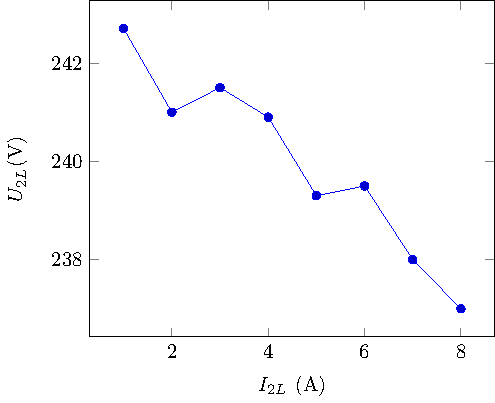
\includegraphics[width=6cm]{fig/r_u2i2.pdf}
	\end{subfigure}
	\caption{SOME CAPTION!}
  \end{figure}



\subsection{Induktive Belastung}
\begin{figure}[H]
    \centering
    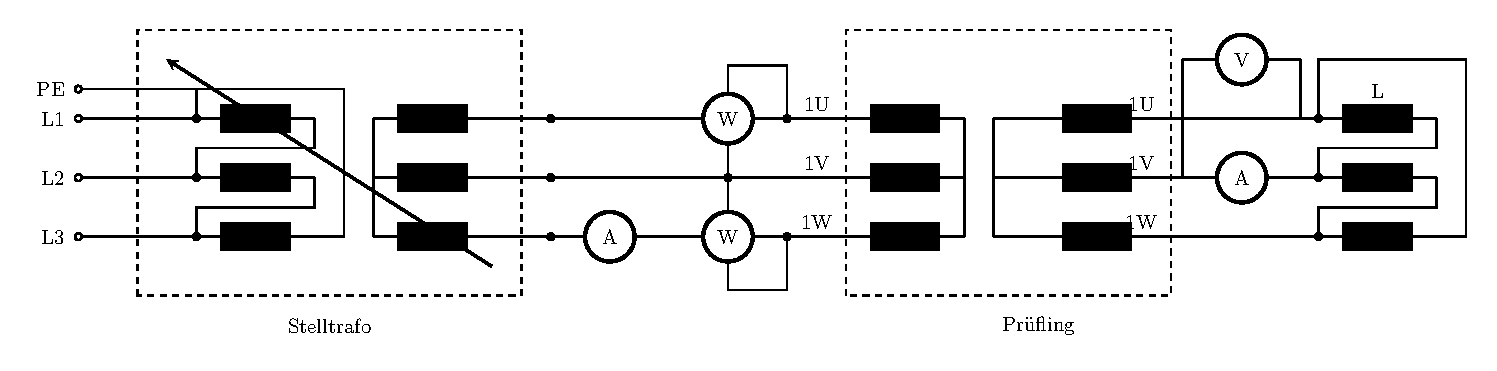
\includegraphics[width=0.95\textwidth]{fig/inductiv_mess.pdf}
    \caption{Messschaltung }
    \label{fig:my_label}
\end{figure}

\begin{figure}[H]
\centering
	\begin{tikzpicture}
		\begin{axis}[
				/pgf/number format/.cd,
				use comma,
				1000 sep={},
				xlabel=$I_{2L} $ (A),
				ylabel={$ U_{2L} \; (\si{\volt})$},
			]
			%The mockup experiment data is stored in a csv file, and imported here.
			\addplot table [x=I_2L (A), y=U_2L, col sep=comma] {data/induk.csv};
			%\addplot table [x=I_2kl, y=I_2kl, col sep=comma] {data/ohmsche_belastung.csv};
		\end{axis}
	\end{tikzpicture}
\end{figure}

\subsection{Kapazitive Belastung}
\begin{figure}[H]
    \centering
    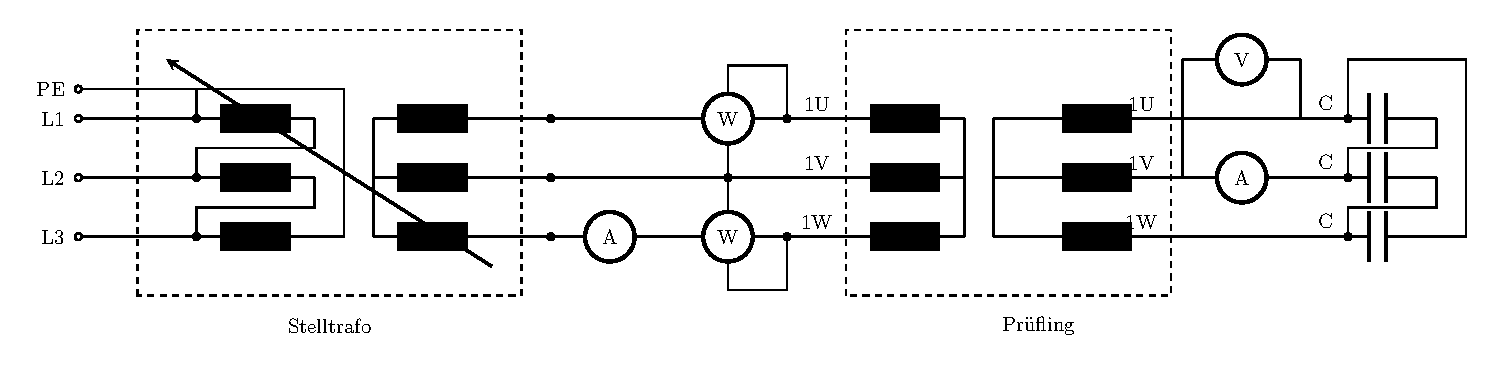
\includegraphics[width=0.95\textwidth]{fig/kap_mess.pdf}
    \caption{Messschaltung }
\end{figure}

\begin{figure}[H]
\centering
	\begin{tikzpicture}
		\begin{axis}[
				/pgf/number format/.cd,
				use comma,
				1000 sep={},
				xlabel=$I_{2L} $ (A),
				ylabel={$ U_{2L} \; (\si{\volt})$},
			]
			%The mockup experiment data is stored in a csv file, and imported here.
			\addplot table [x=I_2L (A), y=U_2L, col sep=comma] {data/kapa.csv};
			%\addplot table [x=I_2kl, y=I_2kl, col sep=comma] {data/ohmsche_belastung.csv};
		\end{axis}
	\end{tikzpicture}
\end{figure}

\subsection{Ersatzschaltbilder und Zeigerbilder}

\begin{figure}[H]
    \centering
    \begin{circuitikz}[thick]

    \coordinate (A) at (0,0);

    \draw (A) to[R,*-,name=R1] ++(3,0) 
    to[european inductor,name=X1] ++ (2,0) 
    to[short] ++(1cm,0) coordinate (m);
    
    \draw (m) to[short,-*] ++(0,-1cm) coordinate (md);
    \draw (md) -- ++ (1.5cm,0) to[european inductor,name=X2] ++(0,-2cm) to[short,-*] ++(-1.5cm,0) coordinate (mdd);
    \draw (md) -- ++ (-1.5cm,0) to[R,name=R2] ++(0,-2cm) to[short,-*] ++(1.5cm,0);
    \draw (mdd) -- ++(0,-1cm) coordinate (d) to[short,-*] (d-|A) coordinate (B);
    \draw (12,0) coordinate (C) to[R,name=R3,*-] ++(-3,0)
     to[european inductor,name=X3,mirror] ++ (-2,0) to[short] ++(-1,0);
    \draw (d) to[short,-*] (d-|C);
    \draw (A) to[open,v=U] (B);
    \draw (C) to[open,v^=U] (C|-B);

    \node[above] at (R1.n){$R_1 = \SI{0.28}{\ohm}$};
    \node[left,xshift=-0.5cm] at (R2.n){$R_{Fe} = \SI{2.55}{\kilo\ohm}$};
    \node[above] at (R3.s){$R^\prime_2 = \SI{0.83}{\ohm}$};
    \node[above] at (X1.n){$ X_{\sigma 1} = \SI{0.5}{\ohm}$ };
    \node[right] at (X2.n){$X_h = \SI{0.49}{\kilo\ohm}$};
    \node[above] at (X3.n){$X^\prime_{\sigma 2} = \SI{0.68}{\ohm}$};


\end{circuitikz}
    \caption{THE EQUIVI CIIIRKKUIT}
    \label{fig:my_label}
\end{figure}





\end{document}